\begin{frame}{$K^0$ kinematical plot with fitting}
  \centering
  $d(K^-, n)"K^0 n"$ looked like 1-step reaction.\\
  2-step like events were observed in IM of $n K^0$ and $"n"$ momentum.\\

  \tminipageThree{
    \begin{figure}
      \includegraphics[width=4cm]{../pic/Run78/KN_ana/fit_KN_IM_npipi_K0_ts_L1520.eps}
    \end{figure}
  }{
    \begin{figure}
      \includegraphics[width=4cm]{../pic/Run78/KN_ana/mmN_mom_IM_npipi_K0.eps}
    \end{figure}
  }{
    \begin{figure}
      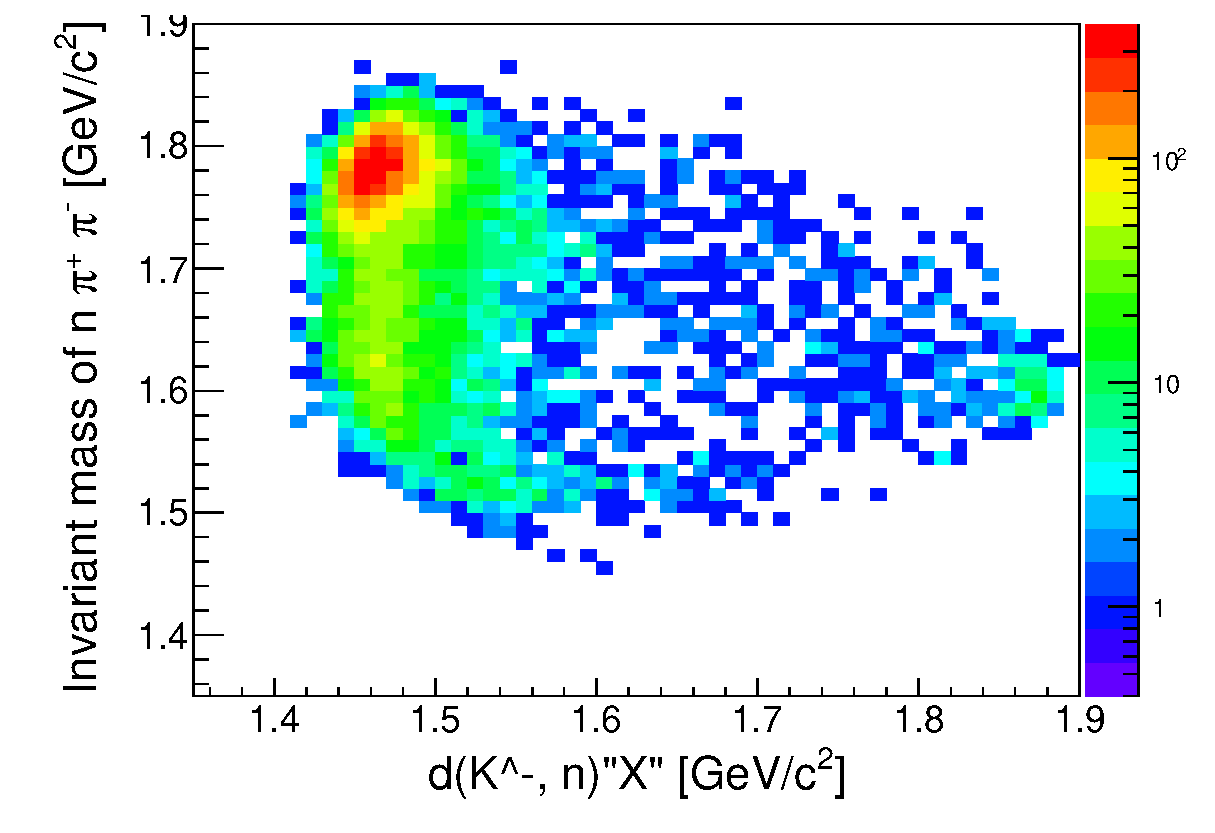
\includegraphics[width=4cm]{../pic/Run78/KN_ana/KN_MM_IM_npipi_K0.eps}
    \end{figure}
  }

  \tminipageThree{
        \scriptsize
    \begin{tikzpicture}
      \begin{feynhand}
        \vertex [particle] (k0) at (-1.5, 1.0) {$K^-$};
        \vertex [particle] (k0_2) at (1.5, 0.35) {$K^0$};
        \vertex [particle] (N)  at (1.5,  1.0) {$n_{detect}$};
        \vertex [particle] (d)  at (-1.5, 0.0) {$d$};
        \vertex [particle] (Nmiss)  at (1.5,  0.0) {$n_{missing}$};
        \vertex (w1) at (0, 0.5);

        \vertex [particle] (dkn)   at (0, 1.0) {$d(K^-, n)"X"$};

        \propag [fermion] (d)  to (w1);
        \propag [fermion] (k0) to (w1);
        \propag [fermion] (w1) to (N);
        \propag [fermion] (w1) to (k0_2);
        \propag [fermion] (d) to (Nmiss);
      \end{feynhand}
    \end{tikzpicture}

        \begin{tikzpicture}
      \begin{feynhand}
        \vertex [particle] (k0) at (-1.5, 1.0) {$K^-$};
        \vertex [particle] (k0_2) at (1.5, 0.2) {$K^0$};
        \vertex [particle] (N)  at (1.5,  1.0) {$n_{detect}$};
        \vertex [particle] (d)  at (-1.5, 0.0) {$d$};
        \vertex [particle] (Kbar)   at (-0.25, 0.02) {$\bar{K}$};
        \vertex [particle] (Nmiss)  at (1.5,  -0.7) {$n_{missing}$};
        \vertex (w1) at (0, 0.3);
        \vertex (w2) at (0,-0.3);

        \vertex [particle] (dkn)   at (0, 1.0) {$d(K^-, n)"X"$};
        \vertex [particle] (IM)   at (1.3, -0.3) {$n K^0 IM$};

	\propag [fermion] (d)  to (w1);
        \propag [fermion] (d)  to (w2);
        \propag [fermion] (k0) to (w1);
        \propag [fermion] (w1) to (N);
        \propag [plain]   (w1) to (w2);
        \propag [fermion] (w2) to (Nmiss);
        \propag [fermion] (w2) to (k0_2);
      \end{feynhand}
    \end{tikzpicture}
  }{
    \begin{figure}
      \includegraphics[width=4cm]{../pic/Run78/KN_ana//fit_mmN_momK0_ts_L1520.eps}
    \end{figure}
  }{
    \begin{figure}
      \includegraphics[width=4cm]{../pic/Run78/KN_ana//fit_KN_MM_K0_ts_L1520.eps}
    \end{figure}
  }

  
\end{frame}
